\documentclass{report}

\newcommand{\name}{\textit{Arcana Azurea Pitou}}
\newcommand{\program}{\textit{NEKO}}

\usepackage[french]{babel}
\usepackage[T1]{fontenc}
\usepackage[utf8]{inputenc}
\usepackage{fontspec}
\usepackage[a4paper]{geometry}
\usepackage{scrextend}
\usepackage{listings}
\usepackage[hidelinks,unicode=true]{hyperref}
\usepackage[pgf]{dot2texi}
\usepackage{pgf}
\usepackage{tikz}
\usepackage{fancyhdr}
\usepackage{sectsty}
\usepackage{titlesec}
\usepackage{csquotes}
\usepackage{hyperref}

\hypersetup{
  colorlinks = true,
  linkcolor = blue,
  urlcolor = blue,
}

\usetikzlibrary{automata}

\pagestyle{fancy}

\fancyhf{}
\lhead{\leftmark}
\rhead{\rightmark}
\rfoot{\thepage}

\setmainfont[
    Path = fonts/sazanami-neko/,
    Extension = .ttf,
    Ligatures = TeX,
    Scale = MatchLowercase,
]{sazanami-mincho}

\setsansfont[
    Path = fonts/sazanami-neko/,
    Extension = .ttf,
    Ligatures = TeX,
    Scale = MatchLowercase,
]{sazanami-gothic}

\title{"neko"}

\author{
   adjivas
   \and
   brezaire
   \and
   flime
   \and
   jpepin
}

\date{}

\begin{document}

\begin{titlepage}
	\centering
	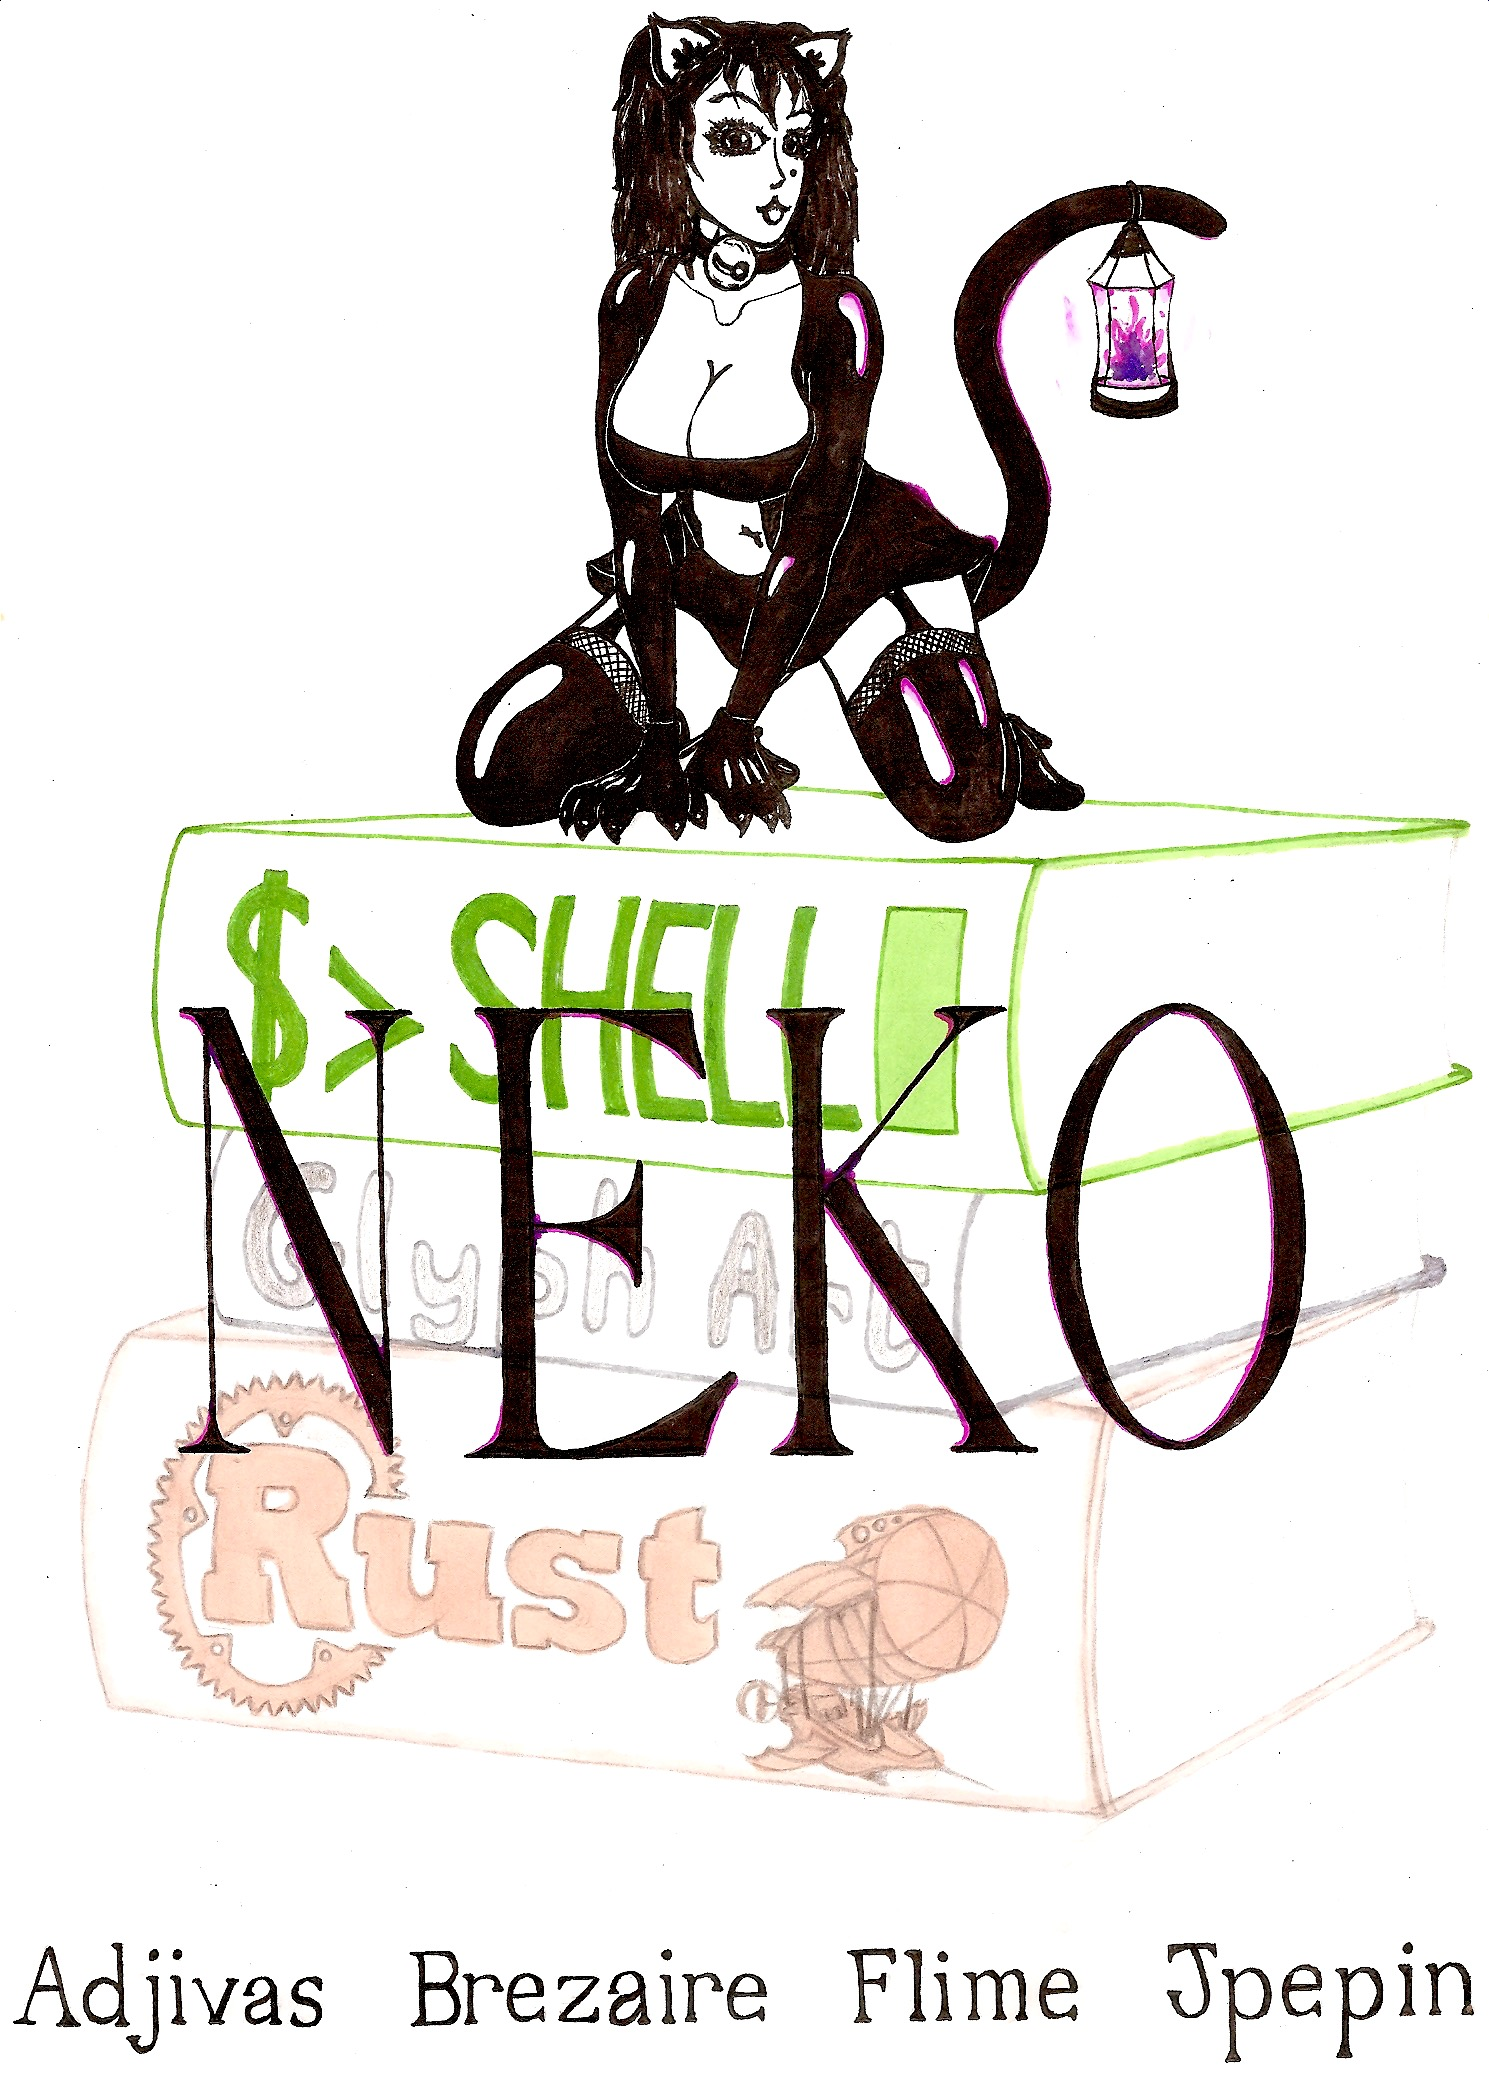
\includegraphics[scale=0.25]{images/neko.jpg}
\end{titlepage}

\tableofcontents

\titleformat{\chapter}[display]
  {\Huge}
  {\filleft\texttt{\chaptertitlename} \Huge\thechapter}
  {0ex}
  {\filleft}
  [\titlerule]

\chapter{Premiere partie}

\section{Préambule}

\begin{figure}[!ht]
  \begin{minipage}{1in}
    \centering
    \fontsize{30pt}{7pt}\selectfont
    \symbol{"E000}\symbol{"E001}\symbol{"E002}\symbol{"E003}\symbol{"E004}\symbol{"E005}\symbol{"E006}\symbol{"E007}\symbol{"E008}\symbol{"E009}\\*
    \symbol{"E00A}\symbol{"E00B}\symbol{"E00C}\symbol{"E00D}\symbol{"E00E}\symbol{"E00F}\symbol{"E010}\symbol{"E011}\symbol{"E012}\symbol{"E013}\\*
    \symbol{"E014}\symbol{"E015}\symbol{"E016}\symbol{"E017}\symbol{"E018}\symbol{"E019}\symbol{"E01A}\symbol{"E01B}\symbol{"E01C}\symbol{"E01D}\\*
    \symbol{"E01E}\symbol{"E01F}\symbol{"E020}\symbol{"E021}\symbol{"E022}\symbol{"E023}\symbol{"E024}\symbol{"E025}\symbol{"E026}\symbol{"E027}\\*
    \symbol{"E028}\symbol{"E029}\symbol{"E02A}\symbol{"E02B}\symbol{"E02C}\symbol{"E02D}\symbol{"E02E}\symbol{"E02F}\symbol{"E030}\symbol{"E031}\\*
  \end{minipage}
  \caption[Caption for LOF]{\href{https://en.wikipedia.org/wiki/Wikipedia:Wikipe-tan}{Wikipe-tan} \textendash{ ウィキペたん }\textendash{ }}
\end{figure}

Une nékoe \textendash{ ねこみみ }\textendash{ } est un persona d'animé japonais avec des traits de chat
\textendash{ mimikko
	\footnote{ Kemonomimi ou mimikko est un personnage humain d'animé avec les caractéristiques d'un animal telles que sa personnalité ou encore son physique
		\textendash{ 獣耳 }\textendash.
			}} \textendash.

Le GlyphArt est l'écriture d'une image via des caractères compris dans l'Unicode privé, ce projet démontre ce procédé via
\href{https://limaconoob.github.io/Image2font}{Image2font}.

$\name$ est une programmeuse nékoe fictive de terminal inventée pour assister son utilisateur.

\section{Introduction}
\thispagestyle{empty}
$\program$ est un prompt nommé $\name$ et qui a pour but d'apporter les Arts, la Culture et une assistance à qui saura utiliser un shell.
Humanisée d’émotions et fondée sur l'expérience de la \href{https://fr.wikipedia.org/wiki/Chambre_chinoise}{chambre chinoise}, celle-ci sera donc instruite via des bibliotèques.

Ce prompt lit sur l'entrée standard, modifie l'interface puis imprime une sortie modifiée selon les bibliotèques fournies qui sera interpretée par le shell parent.

La liste des options est :
\begin{labeling}{Longer label\quad}
	\item[\textbf{
		\textendash p,
		\textendash\textendash from-part <file.neko.part, ...>}] initialise une liste de 
			\textendash{ texels}
				\footnote{ Un texel ou élément de texture est l'unité fondamentale de mesure d'une texture. }
					\textendash { }.
	\item[\textbf{
		\textendash s,
		\textendash\textendash from-sprite <file.neko.sprite, ...>}] initialise une liste de
			\textendash{ sprite}
				\footnote{ Un sprite est une texture délimitée par une surface. }
					\textendash { }.
	\item[\textbf{
		\textendash l,
		\textendash\textendash from-library <[file.so, ...]>
	}] monte dynamiquement une liste de bibliotèques depuis un paquet, un dépôt Git ou un fichier.
\end{labeling}

La liste des options du builtin $\program$ est :

\begin{labeling}{Longer label\quad}
	\item[\textbf{
		\textendash m,
		\textendash\textendash mount <[<name, link, object>, ...]>
	}] monte dynamiquement une liste de bibliotèques depuis un paquet, un dépôt Git ou un fichier.
	\item[\textbf{
		\textendash g,
		\textendash\textendash graphic <position> [<attribut>, ...]
	}] change l'expression de $\name$ .
	\item[\textbf{
		\textendash s,
		\textendash\textendash say <[<sentence>, ...]> <delay=1>
	}] dit une phrase .
	\item[\textbf{
		\textendash c,
		\textendash\textendash call <library> <[<argument>, ...]>
	}] appelle une bibliotèque avec une liste d'arguments .
\end{labeling}

\newpage

\section{Module}

\subsection{Bibliothèque Dynamique}

Ce module est l'interface d'une liste de fonctions externes qui seront dynamiquement chargées depuis des bibliothèques partagées.

Seront executées les séquences suivantes :

\begin{labeling}{Longer label\quad}
	\item[\textbf{Start} quand la bibliothèque est montée.]
	\item[\textbf{Idle} pour chaque cycle.]
	\item[\textbf{MousePress} quand le pointeur est pressé dans le terminal.]
	\item[\textbf{MousePressNeko} quand le pointeur est pressé sur la nékoe.]
	\item[\textbf{MouseRelease} quand le pointeur est relâché dans le terminal.]
	\item[\textbf{MouseReleaseNeko} quand le pointeur est relâché sur la nékoe.]
	\item[\textbf{KeyDown} quand une touche est enfoncée.]
	\item[\textbf{KeyDownRepeat} quand une touche est maintenue enfoncée $\{2\dots{}N\}$.]
	\item[\textbf{KeyDownInterval} durant \textit{KeyDownRepeat}, donne l'intervalle : $\sum_{i=repeat}^{\infty} U_{interval}\times{}i$.]
	\item[\textbf{KeyUp} quand une touche est relâchée.]
	\item[\textbf{Talk} quand une bibliothèque va dire un message.]
	\item[\textbf{Call} pour appeler une bibliothèque avec une liste d'arguments.]
	\item[\textbf{End} quand le processus $\program$ se termine.]
\end{labeling}

Le retour d'une fonction externe peut manipuler les options de builtins tels que \textbf{Graphic}, \textbf{Say} et \textbf{Call}.

\begin{figure}[!ht]
  \centering
  \begin{dot2tex}[dot,scale=0.35]
digraph graphic {
  d2tstyleonly = true;
  node [shape = "box", width = "6", texmode="verbatim", style = "top color=cyan!10,bottom color=cyan!35,draw=cyan!50,rounded corners"];
  graph [shape = "box", texmode="math", style = "top color=blue!10,bottom color=blue!35,draw=blue!50"];

  nodeEvent [label="Struct Event\n
    Func<extern C fn(event: c_int, arg: *const c_char) -> *const c_char>\
	\n
	+ fn new(fun: extern C fn(c_int, *const c_char) -> *const c_char) -> Self
	+ unsafe fn run(&self) -> Vec<&str>
  "];

  nodeLibraryError [label="Enum LibraryError<Display + Debug + Error>\n
    EmptyEvent
	HasOnlyStart
  "];

  nodeLibrary [label="Struct Library<Drop>\n
	start: Option<Event>
	+ idle: Option<Event>
	+ mouse_press: Option<Event>
	+ mouse_press_neko: Option<Event>
	+ mouse_release: Option<Event>
	+ mouse_release_neko: Option<Event>
	+ key_down: Option<Event>
	+ key_down_repeat: Option<Event>
	+ key_down_interval: Option<Event>
	+ key_up: Option<Event>
	call: Option<Event>
	end: Option<Event>\
    \n
	+ fn new(libraryname: &str) -> Result<Self>
  "];

  nodeCompositerError [label="Enum CompositerError<Display + Debug + Error>\n
    badMount(LibraryError)
    UmountNotFound
  "];

  nodeCompositer [label="Struct Compositer<Iterator, Default>\n
    (BinaryHeap<(usize, (Library, String))>)\
	\n
	+ fn mount(libraryname: &str, priority: usize) -> Result<()>
	+ fn unmount(libraryname: &str) -> Result<()>
	+ fn call(libraryname: &str, arguments: Vec<&str>) -> Result<()>
  "];

  nodeEvent -> nodeLibrary
  nodeLibraryError -> nodeLibrary
  nodeLibrary -> nodeCompositer
  nodeCompositerError -> nodeCompositer
}
  \end{dot2tex}
  \caption[Caption for LOF]{ Diagramme UML simplifié du module bibliothèque dynamique. }
  \label{library}
\end{figure}

\newpage

\subsection{Graphique}

Ce module est l'interface d'une liste de primitives telles que des texels et des sprites qui pourront se combiner en nouveaux sprites.

\begin{figure}[!ht]
  \centering
  \begin{dot2tex}[dot,scale=0.35]
digraph graphic {
  d2tstyleonly = true;
  node [shape = "box", width = "4.5", texmode="verbatim", style = "top color=cyan!10,bottom color=cyan!35,draw=cyan!50,rounded corners"];
  graph [shape = "box", texmode="math", style = "top color=blue!10,bottom color=blue!35,draw=blue!50"];

  nodeTexelError [label="Enum TexelError<Display + Debug + Error>\n
    UnknownTexel
    ForbiddenGlyph(char)
  "];

  nodeTexel [label="Enum Texel\n
    EyeLeft(char)
    EyeRight(char)
    EarLeft(char)
    EarRight(char)
    Nose(char)
    Mouth(char)
    Neck(char)
	ShoulderLeft(char)
	ShoulderRight(char)\
    \n
    + new(limb: &str, glyph: char) -> Result<Self>
  "];

  nodeManagerError [label="Enum ManagerError<Display + Debug + Error>\n
      Duplicate
      BadTexel(TexelError)
  "];

  nodeManager [label="Struct Manager<Default>\n
    texel: HashMap<(Posture, Emotion), Texel>
	sprite: HashMap<String, Sprite>\
	\n
    + insert_texel(&mut self, key: (Posture, Emotion), value: Texel) -> Result<()>
	+ insert_sprite(&mut self, key: String, value: Sprite) -> Result<()>
  ", width = 8.5];

  subgraph clusterPostureEmotion {
    nodePosture [label="Enum Posture\n
      LotusHandsOnFloor
      LyingOnSomething
    "];
    nodeEmotion [label="Enum Emotion\n
      Happy
      Malicious
      None
    "];
  }

  nodeSpriteError [label="Enum SpriteError<Display + Debug + Error>\n
    EmptyBoard
  "];

  nodeSprite [label="Struct Sprite\n
    const MAX_X: usize = 7;
    const MAX_Y: usize = 10;
	interval: usize
    sheet: Vec<(Posture, [[(Emotion, Texel); MAX_X]; MAX_Y])>\
    \n
    + new(sheet: Vec<(Posture, [[(Emotion, Texel); MAX_X]; MAX_Y])>, interval: usize) -> Result<Self>
  ", width = 9];

  nodeTexelError -> nodeTexel;
  nodeTexel -> nodeSprite;
  nodeTexel -> nodeManager;
  nodeManagerError -> nodeManager;
  nodePosture -> nodeSprite;
  nodePosture -> nodeManager;
  nodeEmotion -> nodeSprite;
  nodeEmotion -> nodeManager;
  nodeSpriteError -> nodeSprite;
  nodeSprite -> nodeManager;
}
  \end{dot2tex}
  \caption[Caption for LOF]{ Diagramme UML \footnotemark{} simplifié du module graphique. }
  \label{graphic}
\end{figure}

\footnotetext{En génie logiciel, le langage de modélisation orienté objet unifié de l'anglais
	\enquote{Unified Modeling Language}
		\textendash{ UML }\textendash{ } est la représentation schématique d'un programme par de l'orienté objet}

\chapter{Deuxieme partie}

\section{Bibliothèque}

Ce chapitre énumère une liste exhaustive de bibliothèques dynamiques issues de langages Libres et qui seront programmées par \enquote{la confrérie des ténèbres} pour apporter une base à ce qui à pour but de s'étendre et évoluer grâce à la communauté.\\*

\begin{labeling}{Longer label\quad}
    \item[\textbf{help-git} \enquote{noob}] Si l'utilisateur utilise plus d'une fois sans succès l'option \textit{push}, la nékoe proposera son aide puis informera des instructions shell à saisir.
	\item[\textbf{travis-git} \enquote{assistance, information}] Quand l'utilisateur publie une nouvelle version de sa branche et qu'un fichier \textit{.travis} est défini à la racine du projet, alors la nékoe informera son utilisateur du résultat.
    \item[\textbf{must-sleep} \enquote{medical}] Quand l'utilisateur dépasse dix heures d'activités, la nékoe aura des signes de fatigue et informera une seule fois des conséquences du manque de sommeil sur la productivité.
    \item[\textbf{lock-terminal} \enquote{assistance}] Après N secondes d'inactivité, la nékoe verrouille le terminal et vit sa vie.
	\item[\textbf{help-stackoverflow} \enquote{assistance, information}] Si un programme affiche une erreur, la nékoe essaie une recherche sur StackOverflow et propose d'informer l'utilisateur si elle a trouvé une solution.
	\item[\textbf{repos-dex} \enquote{assistance, information}] Quand l'utilisateur entre dans un projet, la nékoe fournit une description.
	\item[\textbf{email} \enquote{information}] Quand l'utilisateur reçoit un courriel, la nékoe proposera de le lire.
	\item[\textbf{man-description} \enquote{help, information}] Lorsque l'utilisateur saisit la commande \textit{man}, la nékoe avant la validation de ce dernier l'informe de la description de la commande.
	\item[\textbf{hungry} \enquote{social}] Si l'utilisateur clique sur la nékoe, celle-ci prend une expression affamée.
	\item[\textbf{not-leave-me} \enquote{social}] Pendant que l'utilisateur saisit la commande \textit{exit}, la nékoe essaie des stratagèmes pour ne pas être abandonnée.
	\item[\textbf{overload} \enquote{social, information}] La lanterne clignote lorsque l'utilisateur surcharge le CPU.
	\item[\textbf{season} \enquote{social}] La nékoe sera plus vêtue en hiver qu'en été.
	\item[\textbf{hello} \enquote{social}] La nékoe salue son utilisateur au lancement du terminal.
	\item[\textbf{wait-make} \enquote{social}] Durant une compilation, la nékoe distraira l'utilisateur avec des histoires.
	\item[\textbf{orphan-file} \enquote{noob, information}] Avant de saisir une publication, la nékoe avertie de la présence de fichiers orphelins.
	\item[\textbf{gitignore} \enquote{assistance}] À la création d'un projet, la nékoe propose de créer un .gitignore.
\end{labeling}

\end{document}
